\documentclass{beamer}
\usepackage[utf8]{inputenc}
\usepackage[T1]{fontenc}
\usepackage[french]{babel}
\usepackage{amsmath,amsfonts,amssymb}
\usepackage{graphicx}

\usetheme{Warsaw}

\author{Aurèle Barrière \& Nathan Thomasset}
\title{Cryptographie}
\date{10 mars 2016}


\begin{document}

\begin{frame}
\maketitle
\end{frame}

\begin{frame}{Mise en situation}
  Iseut souhaite envoyer des messages d'amour à Tristan, qui vit en Bretagne avec sa femme. Bien évidemment il ne faut pas que cette dernière puisse les lire, ce qui créerait une situation quelque peu inconfortable.
  \begin{block}{}
   Comment faire pour s'assurer de pouvoir communiquer impunément ?
   \end{block}

  \end{frame}

\begin{frame}{Intérêt de la cryptographie}
  \begin{itemize}
  \item Cartes bleues
    
  \item Mail
    
  \item Transactions bancaires
  
  \item Chiffrement des données sensibles (militaires ou privées)
\end{itemize}
\end{frame}

\begin{frame}{Un codage ultime?}
  Seul quelqu'un qui connaitraît la clé pourrait décoder : est-ce réellement possible ?

Cryptographie symétrique : on a tous les deux une même clé.
\begin{figure}
\centering
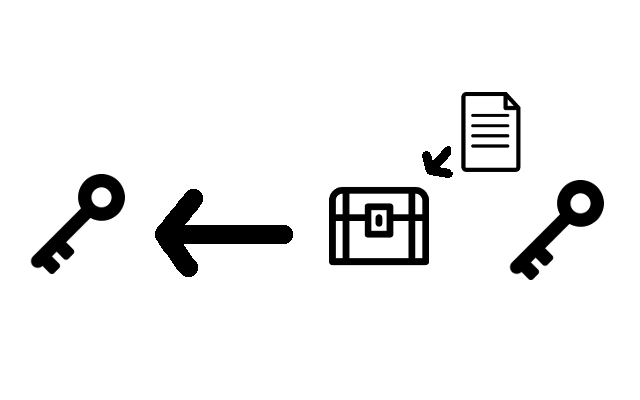
\includegraphics[scale = 0.4]{symetric.png}
\end{figure}
  \end{frame}

\begin{frame}{Exemple : chiffrement de César}
  Décalage constant. 
$$A\rightarrow B, B\rightarrow C, \text{...}$$ 
$$A\rightarrow C, B\rightarrow D, \text{...}$$

  \begin{figure}
    \centering
  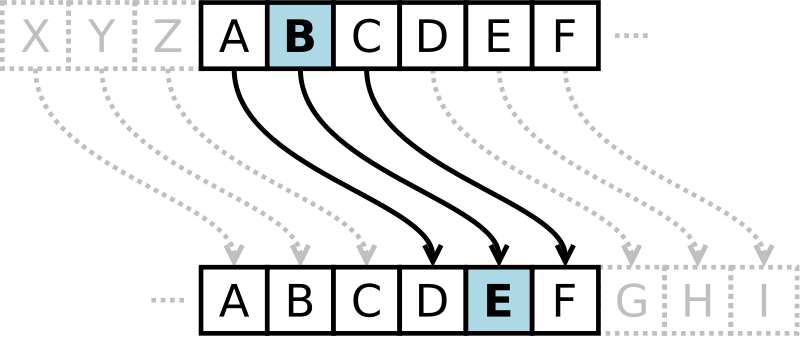
\includegraphics[scale = 0.25]{cesar.png}
\end{figure}
\end{frame}


\begin{frame}{Casser le code de César}
\begin{block}{}
  26 décalages possibles.\\
  Mot à décrypter :  iravivqvqrpelcgv 
\end{block}
  

\footnotesize
\begin{tabular}{c c}
jsbwjwrwrsqfmdhw &  
ktcxkxsxstrgneix\\
ludylytytushofjy &  
mvezmzuzuvtipgkz\\
nwfanavavwujqhla &   
oxgbobwbwxvkrimb\\
pyhcpcxcxywlsjnc & 
qzidqdydyzxmtkod\\
rajerezezaynulpe &
sbkfsfafabzovmqf\\
tclgtgbgbcapwnrg &
udmhuhchcdbqxosh\\
\textbf{\textcolor{red!60!black}{venivididecrypti}} &
wfojwjejefdszquj\\
xgpkxkfkfgetarvk &
yhqlylglghfubswl\\
zirmzmhmhigvctxm &
ajsnaninijhwduyn\\
bktobojojkixevzo &
clupcpkpkljyfwap\\
dmvqdqlqlmkzgxbq &
enwrermrmnlahycr\\
foxsfsnsnombizds &
gpytgtotopncjaet\\
hqzuhupupqodkbfu &
iravivqvqrpelcgv\\
\end{tabular}
\normalsize
  \end{frame}

\begin{frame}{Énumération des clés}
  Énumérer les clés possibles (décalages). Regarder tous les résultats.

  \begin{figure}
    \centering
    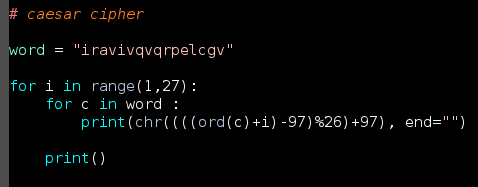
\includegraphics[scale = 0.6]{cesarcode.png}
\end{figure}

\begin{block}{}
Ensemble de clés fini
\end{block}

  \end{frame}

%\begin{frame}{Complexité}
 % Le calcul, c'est pas gratuit.

  %Trop de clés $\Rightarrow$ trop de calcul, trop de résultats
%\end{frame}

%\begin{frame}{Énumération des clés}
  %\begin{itemize}
  
  %\item Il est possible d'énumérer toutes les clés.
  
  %\item Dans la majorité des algorithmes employés, l'ensemble des clés est fini.
  
  %\item Même si ce n'est pas le cas, la mémoire allouée au stockage de la clé est limitée : l'ensemble des clés utilisables est fini.
  
  %\end{itemize}
  %\end{frame}

\begin{frame}{Complexité}

  \begin{alertblock}{Le calcul, c'est pas gratuit}
    Trop de clés $\Rightarrow$ trop de calcul, trop de résultats
\end{alertblock}
  L'objectif n'est pas de créer un chiffrement incassable, mais un chiffrement qui soit trop coûteux à casser.

  
  \begin{figure}
  \centering
  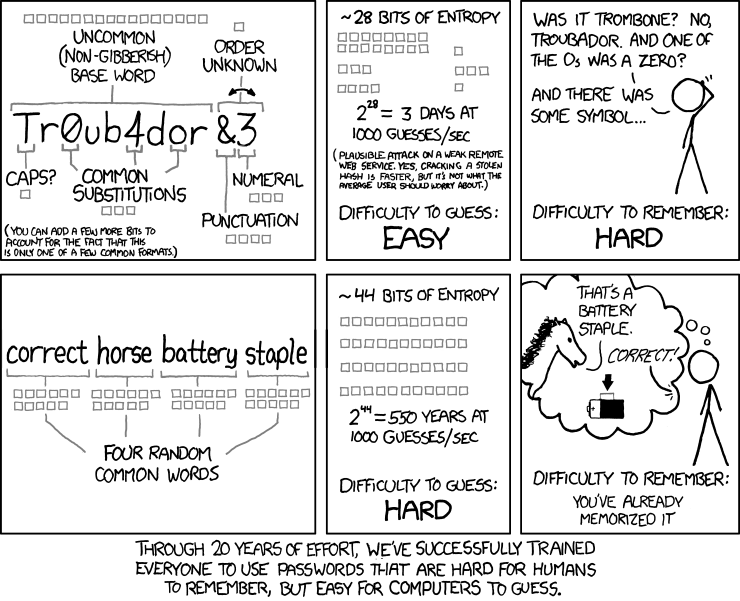
\includegraphics[scale = 0.3]{xkcdpassword_strength.png}
  \end{figure}
  \end{frame}

\begin{frame}{D'autres exemples}
  Hill

  Vigenere
  \end{frame}

\begin{frame}{Analyse fréquentielle}
  Chiffres pour matrices de Hill

  Fréquences français
  \end{frame}


\begin{frame}{Cryptographie asymétrique}
  Tristan a perdu la clé. Ne pouvant pas la faire refaire, il leur faut trouver un nouveau moyen de communiquer.
\end{frame}

\begin{frame}{RSA}
  Schéma
  \end{frame}

\begin{frame}{Limites}
  \begin{figure}
    \centering
    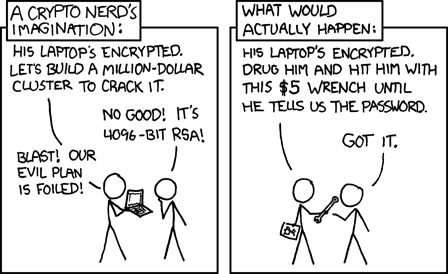
\includegraphics[scale = 0.5]{xkcdsecurity.png}
  \end{figure}
\end{frame}

\begin{frame}{Ressources et idées}
  GPG mail
  
  sources des images
  \end{frame}





\end{document}
